% !TEX root=./adl.tex

% -----------------------------------------------------------------------
\section{Multimodal Models}

% =======================================================================
\subsection{From Language to Vision-Language}

% -----------------------------------------------------------------------
\begin{frame}{Motivation: Why Multimodal?}

  Large language models understand text, but the world is \emph{multimodal}: images, video, audio, \ldots

  \vspace{0.4em}
  \begin{columns}
    \begin{column}{0.48\textwidth}
      \textbf{Key questions}:
      \begin{itemize}
        \item Can we learn \emph{joint} representations of images and text?
        \item Can a model \emph{reason} about images using language?
        \item Can we leverage web-scale image-text data?
      \end{itemize}
    \end{column}
    \begin{column}{0.48\textwidth}
      \textbf{Two paradigms}:
      \begin{description}[style=nextline]
        \item[Contrastive alignment] Shared embedding space for images and text (CLIP, SigLIP)
        \item[Generative VLM] Visual features fed into a language model that \emph{generates} text (PaliGemma, LLaVA)
      \end{description}
    \end{column}
  \end{columns}

  \vspace{0.3em}
  \begin{center}
    \begin{tikzpicture}[
      scale=0.92, every node/.style={scale=0.92},
      box/.style={draw, rounded corners, minimum width=1.6cm, minimum height=0.5cm, align=center, font=\scriptsize},
      capbox/.style={draw, rounded corners, fill=cyan!12, align=center, font=\scriptsize, inner sep=2pt},
      arr/.style={-Stealth, semithick},
      % a small illustrative photo (dog on grass, sun)
      photo/.pic={
        \begin{scope}
          \clip (0,0) rectangle (1,0.8);
          \fill[blue!22] (0,0) rectangle (1,0.8);
          \fill[green!45!brown!35] (0,0) rectangle (1,0.30);
          \fill[yellow!75!orange] (0.80,0.62) circle (0.10);
          % dog
          \fill[brown!55] (0.40,0.16) ellipse (0.13 and 0.065);
          \fill[brown!55] (0.535,0.215) circle (0.058);
          \fill[brown!45] (0.30,0.10) -- (0.27,0.04) -- (0.34,0.10) -- cycle;
          \fill[brown!45] (0.49,0.105) -- (0.52,0.04) -- (0.55,0.11) -- cycle;
        \end{scope}
        \draw[thick] (0,0) rectangle (1,0.8);
      },
    ]
      % ===================== LEFT : CONTRASTIVE =====================
      \node[font=\small\bfseries, text=orange!60!black] at (-3.3,3.35) {Contrastive (CLIP / SigLIP)};

      \path (-5.15,1.95) pic {photo};
      \node[capbox, text width=1.4cm] (lcap) at (-1.9,2.35) {``a dog on the grass''};

      \node[box, fill=orange!22] (lienc) at (-4.65,0.85) {Image\\Encoder};
      \node[box, fill=cyan!25]   (ltenc) at (-1.9,0.85)  {Text\\Encoder};
      \draw[arr] (-4.65,1.95) -- (lienc);
      \draw[arr] (lcap) -- (ltenc);

      % embedding vectors meeting
      \node[draw, circle, fill=orange!12, inner sep=1.5pt, font=\scriptsize] (li) at (-4.0,-0.45) {$\mathbf{I}$};
      \node[draw, circle, fill=cyan!15,  inner sep=1.5pt, font=\scriptsize] (lt) at (-2.55,-0.45) {$\mathbf{T}$};
      \draw[arr] (lienc) -- (li);
      \draw[arr] (ltenc) -- (lt);
      \draw[<->, semithick, violet] (li) -- (lt);
      \node[font=\scriptsize, text=violet!65!black, align=center] at (-3.3,-1.25)
        {pull matching\\$\cos(\mathbf{I},\mathbf{T})$ together};

      % divider
      \draw[gray!40, dashed] (0,-1.6) -- (0,3.0);

      % ===================== RIGHT : GENERATIVE =====================
      \node[font=\small\bfseries, text=green!50!black] at (3.4,3.35) {Generative (PaliGemma / LLaVA)};

      % image branch (vertical, x = 1.8)
      \path (1.30,1.95) pic {photo};
      \node[box, fill=orange!22] (rienc) at (1.8,1.05)  {Image Enc.};
      \node[box, fill=green!18]  (rproj) at (1.8,-0.10) {Projection};
      \draw[arr] (1.8,1.95) -- (rienc);
      \draw[arr] (rienc) -- (rproj);

      % prompt above LLM (vertical) ; LLM aligned with projection (horizontal)
      \node[capbox] (rprompt) at (4.4,1.4) {``Describe.''};
      \node[box, fill=blue!16, minimum width=1.7cm, minimum height=1.1cm] (rllm) at (4.4,-0.10) {LLM};
      \draw[arr] (rproj.east) -- (rllm.west);
      \draw[arr] (rprompt) -- (rllm);

      % output below LLM (vertical)
      \node[capbox, fill=green!20, text width=2.3cm] (rout) at (4.4,-1.4)
        {``A dog sitting on the grass.''};
      \draw[arr, green!45!black] (rllm) -- (rout);
    \end{tikzpicture}
  \end{center}
\end{frame}

% =======================================================================
\subsection{CLIP}

% -----------------------------------------------------------------------
\begin{frame}{CLIP: Contrastive Language-Image Pre-training}

  \cite{radford2021clip}: Learn visual representations from \textbf{natural language supervision} instead of fixed label sets.

  \vspace{0.5em}
  \textbf{Core idea}: Train two encoders (image + text) so that matching pairs have high cosine similarity in a shared embedding space.

  \vspace{0.3em}
  \begin{center}
    \begin{tikzpicture}[
      scale=0.92, every node/.style={scale=0.92},
      enc/.style={draw, rounded corners, minimum width=1.7cm, minimum height=0.55cm, align=center, font=\scriptsize},
      capbox/.style={draw, rounded corners, fill=cyan!12, align=center, font=\scriptsize, inner sep=2.5pt},
      arr/.style={-Stealth, semithick},
      photo/.pic={
        \begin{scope}
          \clip (0,0) rectangle (1,0.8);
          \fill[blue!22] (0,0) rectangle (1,0.8);
          \fill[green!45!brown!35] (0,0) rectangle (1,0.30);
          \fill[yellow!75!orange] (0.80,0.62) circle (0.10);
          \fill[brown!55] (0.40,0.16) ellipse (0.13 and 0.065);
          \fill[brown!55] (0.535,0.215) circle (0.058);
          \fill[brown!45] (0.30,0.10) -- (0.27,0.04) -- (0.34,0.10) -- cycle;
          \fill[brown!45] (0.49,0.105) -- (0.52,0.04) -- (0.55,0.11) -- cycle;
        \end{scope}
        \draw[thick] (0,0) rectangle (1,0.8);
      },
    ]
      % ---- inputs ----
      \path (-6.0,0.9) pic {photo};
      \node[capbox, text width=1.7cm] at (-5.5,-1.3) {``a dog on the grass''};

      % ---- encoders ----
      \node[enc, fill=orange!22] (ienc) at (-3.3,1.3) {Image Encoder};
      \node[font=\tiny, text=gray] at (-3.3,0.72) {ViT / ResNet};
      \node[enc, fill=cyan!25]   (tenc) at (-3.3,-1.3) {Text Encoder};
      \node[font=\tiny, text=gray] at (-3.3,-1.88) {Transformer};
      \draw[arr] (-5.5,1.3) -- (ienc);
      \draw[arr] (-5.5,-1.3) -- (tenc);

      % ---- projections ----
      \node[enc, fill=orange!12, minimum width=1.3cm] (iproj) at (-1.2,1.3) {Linear\\Proj.};
      \node[enc, fill=cyan!12, minimum width=1.3cm]  (tproj) at (-1.2,-1.3) {Linear\\Proj.};
      \draw[arr] (ienc) -- (iproj);
      \draw[arr] (tenc) -- (tproj);

      % ---- shared embedding space panel ----
      \def\ox{2.2}\def\oy{-0.65}          % origin of the vector plot
      \draw[rounded corners, draw=violet!40, fill=violet!4]
        (0.5,-1.7) rectangle (4.6,1.85);
      \node[font=\scriptsize\bfseries, text=violet!60!black] at (2.55,1.6) {shared embedding space};

      % light axes
      \draw[gray!45, -Stealth] (\ox,\oy) -- (\ox+2.0,\oy);
      \draw[gray!45, -Stealth] (\ox,\oy) -- (\ox,\oy+2.0);

      % the two feature vectors (small angle = high similarity)
      \draw[-Stealth, very thick, orange!80!black] (\ox,\oy) -- ++(65:1.85)
        node[above right=-2pt, font=\scriptsize, text=orange!70!black] {$\mathbf{I}$};
      \draw[-Stealth, very thick, cyan!70!black] (\ox,\oy) -- ++(48:1.7)
        node[right=0pt, font=\scriptsize, text=cyan!60!black] {$\mathbf{T}$};
      % angle arc
      \draw[violet, semithick] (\ox,\oy)+(48:0.65) arc (48:65:0.65);
      \node[font=\tiny, text=violet] at (\ox+0.78,\oy+0.72) {$\theta$};

      % feed projections into the panel
      \draw[arr, orange!70!black] (iproj) to[out=0,in=150] (\ox-0.05,\oy+0.7);
      \draw[arr, cyan!60!black]  (tproj) to[out=0,in=210] (\ox-0.05,\oy+0.1);

      % similarity formula
      \node[font=\scriptsize, align=center] at (2.55,-2.4)
        {$\cos\theta=\dfrac{\mathbf{I}\cdot\mathbf{T}}{\lVert\mathbf{I}\rVert\,\lVert\mathbf{T}\rVert}$\quad
         small angle $\Rightarrow$ high similarity};
    \end{tikzpicture}
  \end{center}

  \vspace{0.6em}
  \begin{itemize}
    \item \textbf{Dataset}: 400M image-text pairs from the web (WebImageText)
    \item \textbf{Encoders}: ViT (best: ViT-L/14) or ResNet for images; Transformer for text
    \item Both encoders project into a shared $d$-dimensional space via learned linear projections
  \end{itemize}
\end{frame}

% -----------------------------------------------------------------------
\begin{frame}{CLIP: Encoder Architectures}

  Both towers are trained \textbf{from scratch} (no ImageNet / LM pretraining).

  \vspace{0.3em}
  \begin{columns}
    \begin{column}{0.52\textwidth}
      \textbf{Image encoder} (two families studied):
      \begin{description}[style=nextline, leftmargin=0.6em]
        \item[Modified ResNet]
          \begin{itemize}
            \item ResNet-D tweaks~\cite{he2019bagoftricks} + antialiased (blur) pooling
            \item Global average pool replaced by \textbf{attention pooling} (one multi-head attention layer, query = pooled feature)
            \item EfficientNet-style scaling: RN50, RN50x4, RN50x16, RN50x64
          \end{itemize}
        \item[Vision Transformer]
          \begin{itemize}
            \item ViT-B/32, ViT-B/16, ViT-L/14
            \item Extra LayerNorm on patch + position embeddings
            \item \textbf{Best}: ViT-L/14, then fine-tuned 1 epoch at \textbf{336px} (ViT-L/14@336px)
          \end{itemize}
      \end{description}
    \end{column}
    \begin{column}{0.46\textwidth}
      \textbf{Text encoder}:
      \begin{itemize}
        \item Transformer (GPT-2 style), \textbf{causal} masked self-attention
        \item 63M params: 12 layers, width 512, 8 heads
        \item Lower-cased \textbf{BPE}, vocab 49{,}152; sequence capped at \textbf{76} tokens, bracketed by \texttt{[SOS]}/\texttt{[EOS]}
        \item Feature = final-layer activation at \texttt{[EOS]} $\to$ LayerNorm
      \end{itemize}

      \vspace{0.4em}
      \textbf{Projection head}:
      \begin{itemize}
        \item Each tower mapped to the shared space by a \textbf{single linear} projection
        \item A non-linear projection head did \emph{not} help (unlike SimCLR)
      \end{itemize}
    \end{column}
  \end{columns}
\end{frame}

% -----------------------------------------------------------------------
\begin{frame}{CLIP: Contrastive Loss}

  Given a batch of $N$ image-text pairs, CLIP computes an $N \times N$ matrix of scaled cosine similarities:
  \[
      \ell_{ij} = \frac{\mathbf{I}_i \cdot \mathbf{T}_j}{\norm{\mathbf{I}_i} \cdot \norm{\mathbf{T}_j} \cdot \tau}
  \]
  where $\tau$ is a \textbf{learnable temperature} parameter (log-parameterized, initialized to $\nicefrac{1}{0.07}$).

  \vspace{0.3em}
  The loss is a \textbf{symmetric cross-entropy} over this matrix:
  \begin{align*}
    \mathcal{L}_{\text{img}} &= -\frac{1}{N} \sum_{i=1}^{N} \log \frac{\exp(\ell_{ii})}{\sum_{j=1}^{N} \exp(\ell_{ij})}
    & \text{(image} \to \text{text)} \\[4pt]
    \mathcal{L}_{\text{txt}} &= -\frac{1}{N} \sum_{j=1}^{N} \log \frac{\exp(\ell_{jj})}{\sum_{i=1}^{N} \exp(\ell_{ij})}
    & \text{(text} \to \text{image)} \\[4pt]
    \mathcal{L}_{\text{CLIP}} &= \tfrac{1}{2}\bigl(\mathcal{L}_{\text{img}} + \mathcal{L}_{\text{txt}}\bigr)
  \end{align*}

  \begin{itemize}
    \item Ground truth: the \textbf{diagonal} of the $N \times N$ matrix (matching pairs)
    \item Each row = $N$-way classification: ``which text matches this image?''
    \item Each column = $N$-way classification: ``which image matches this text?''
    \item Large batch size ($N = 32{,}768$) is critical: more negatives $\Rightarrow$ better representations
  \end{itemize}
\end{frame}

% -----------------------------------------------------------------------
\begin{frame}{CLIP: Contrastive Loss and Similarity Matrix}

  \begin{center}
    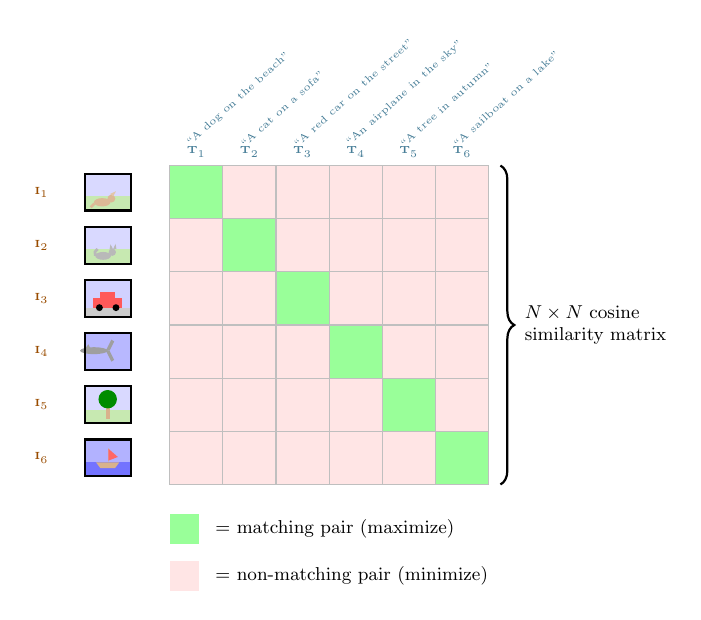
\begin{tikzpicture}[scale=0.75, every node/.style={scale=0.75},
      % ---- tiny scene icons, each drawn in a (0,0)-(1,0.8) box ----
      icondog/.pic={
        \fill[blue!15](0,0)rectangle(1,.8); \fill[green!50!brown!35](0,0)rectangle(1,.32);
        \fill[brown!55](.38,.18)ellipse(.18 and .09); \fill[brown!55](.58,.26)circle(.085);
        \fill[brown!45](.62,.31)--(.68,.42)--(.55,.36)--cycle;
        \draw[brown!55,line width=1pt](.21,.15)--(.13,.07);
        \draw[thick](0,0)rectangle(1,.8);},
      iconcat/.pic={
        \fill[blue!15](0,0)rectangle(1,.8); \fill[green!50!brown!35](0,0)rectangle(1,.32);
        \fill[gray!55](.4,.17)ellipse(.17 and .085); \fill[gray!55](.6,.25)circle(.08);
        \fill[gray!55](.54,.31)--(.56,.42)--(.61,.33)--cycle;
        \fill[gray!55](.62,.32)--(.67,.43)--(.69,.32)--cycle;
        \draw[gray!55,line width=1pt](.23,.17)to[out=110,in=200](.28,.32);
        \draw[thick](0,0)rectangle(1,.8);},
      iconcar/.pic={
        \fill[blue!18](0,0)rectangle(1,.8); \fill[gray!40](0,0)rectangle(1,.2);
        \fill[red!65](.18,.2)rectangle(.82,.4); \fill[red!65](.34,.4)rectangle(.66,.54);
        \fill[black](.32,.2)circle(.075); \fill[black](.68,.2)circle(.075);
        \draw[thick](0,0)rectangle(1,.8);},
      iconplane/.pic={
        \fill[blue!28](0,0)rectangle(1,.8);
        \fill[gray!75](.2,.42)ellipse(.3 and .075);
        \fill[gray!75](.46,.42)--(.58,.66)--(.64,.62)--(.54,.42)--cycle;
        \fill[gray!75](.46,.42)--(.58,.18)--(.64,.22)--(.54,.42)--cycle;
        \fill[gray!75](-.02,.42)--(.08,.56)--(.13,.46)--cycle;
        \draw[thick](0,0)rectangle(1,.8);},
      icontree/.pic={
        \fill[blue!15](0,0)rectangle(1,.8); \fill[green!50!brown!35](0,0)rectangle(1,.28);
        \fill[brown!60](.46,.1)rectangle(.54,.44); \fill[green!55!black](.5,.52)circle(.2);
        \draw[thick](0,0)rectangle(1,.8);},
      iconboat/.pic={
        \fill[blue!30](0,0)rectangle(1,.8); \fill[blue!55](0,0)rectangle(1,.3);
        \fill[brown!60](.25,.3)--(.75,.3)--(.66,.18)--(.34,.18)--cycle;
        \fill[gray!50,line width=.8pt](.5,.3)rectangle(.515,.62);
        \fill[red!60](.515,.34)--(.515,.6)--(.72,.42)--cycle;
        \draw[thick](0,0)rectangle(1,.8);},
    ]
      \def\n{6}
      \def\s{0.9}
      \def\thsc{0.78}   % thumbnail scale

      % Column labels: realistic image captions
      \foreach \j/\w in {1/{A dog on the beach},2/{A cat on a sofa},3/{A red car on the street},4/{An airplane in the sky},5/{A tree in autumn},6/{A sailboat on a lake}} {
        \node[font=\tiny, text=cyan!55!black, rotate=42, anchor=south west]
          at ({(\j-0.5)*\s-0.10}, {\n*\s + 0.12}) {``\w''};
        \node[font=\tiny, text=cyan!55!black, anchor=south]
          at ({(\j-0.5)*\s}, {\n*\s + 0.02}) {$\mathbf{T}_{\j}$};
      }
      % Row labels: tiny scene images
      \foreach \i/\name in {1/icondog,2/iconcat,3/iconcar,4/iconplane,5/icontree,6/iconboat} {
        \pgfmathsetmacro{\cy}{(\n - \i + 0.5)*\s}
        \path ({-1.05 - \thsc*0.5}, {\cy - \thsc*0.4}) pic[scale=\thsc] {\name};
        \node[font=\tiny, text=orange!60!black, anchor=east] at (-1.15-\thsc, \cy) {$\mathbf{I}_{\i}$};
      }

      % Grid with diagonal highlighted
      \foreach \i in {1,...,\n} {
        \foreach \j in {1,...,\n} {
          \pgfmathtruncatemacro{\isdiag}{\i == \j ? 1 : 0}
          \ifnum\isdiag=1
            \fill[green!40] ({(\j-1)*\s}, {(\n-\i)*\s}) rectangle ++(\s, \s);
            \node[font=\small\bfseries] at ({(\j-0.5)*\s}, {(\n-\i+0.5)*\s}) {\checkmark};
          \else
            \fill[red!10] ({(\j-1)*\s}, {(\n-\i)*\s}) rectangle ++(\s, \s);
          \fi
          \draw[gray!50] ({(\j-1)*\s}, {(\n-\i)*\s}) rectangle ++(\s, \s);
        }
      }

      % Brace and label right
      \draw[decorate, decoration={brace, amplitude=5pt}, thick]
        ({\n*\s + 0.2}, {\n*\s}) -- ({\n*\s + 0.2}, 0)
        node[midway, right=8pt, font=\small, align=left] {$N \times N$ cosine\\similarity matrix};

      % Legend
      \fill[green!40] (0, -1.0) rectangle ++(0.5, 0.5);
      \node[font=\small, anchor=west] at (0.65, -0.75) {= matching pair (maximize)};
      \fill[red!10] (0, -1.8) rectangle ++(0.5, 0.5);
      \node[font=\small, anchor=west] at (0.65, -1.55) {= non-matching pair (minimize)};
    \end{tikzpicture}
  \end{center}

  \vspace{0.3em}
  Each row and each column is treated as an independent $N$-way softmax classification.
  The model learns to push matching pairs (diagonal) together and non-matching pairs apart.
\end{frame}

% -----------------------------------------------------------------------
\begin{frame}{CLIP: Zero-Shot Image Classification}

  CLIP enables \textbf{zero-shot classification} without any task-specific training:

  \vspace{0.2em}
  \begin{center}
    \begin{tikzpicture}[
      scale=0.9, every node/.style={scale=0.9},
      enc/.style={draw, rounded corners, fill=orange!18, minimum width=1.6cm, minimum height=0.55cm, align=center, font=\scriptsize},
      prompt/.style={draw, rounded corners, fill=cyan!12, align=center, font=\tiny, inner sep=2pt, text width=1.9cm, minimum height=0.4cm},
      arr/.style={-Stealth, semithick},
      photo/.pic={
        \begin{scope}
          \clip (0,0) rectangle (1,0.8);
          \fill[blue!22] (0,0) rectangle (1,0.8);
          \fill[green!45!brown!35] (0,0) rectangle (1,0.30);
          \fill[yellow!75!orange] (0.80,0.62) circle (0.10);
          \fill[brown!55] (0.40,0.16) ellipse (0.13 and 0.065);
          \fill[brown!55] (0.535,0.215) circle (0.058);
          \fill[brown!45] (0.30,0.10) -- (0.27,0.04) -- (0.34,0.10) -- cycle;
          \fill[brown!45] (0.49,0.105) -- (0.52,0.04) -- (0.55,0.11) -- cycle;
        \end{scope}
        \draw[thick] (0,0) rectangle (1,0.8);
      },
    ]
      % ---- image branch (top) ----
      \path (-6.4,1.5) pic {photo};
      \node[font=\tiny, text=gray, anchor=north] at (-5.9,1.45) {test image};
      \node[enc, fill=orange!22] (ienc) at (-3.7,1.9) {Image Encoder};
      \draw[arr] (-5.4,1.9) -- (ienc);

      % ---- text branch (bottom): all prompts -> one text encoder ----
      \node[prompt] (p1) at (-6.0,-0.1)  {``a photo of a \textbf{dog}''};
      \node[prompt] (p2) at (-6.0,-0.8)  {``a photo of a \textbf{cat}''};
      \node[prompt] (p3) at (-6.0,-1.5)  {``a photo of a \textbf{car}''};
      \node[prompt] (p4) at (-6.0,-2.2)  {``a photo of a \textbf{plane}''};
      \node[enc, fill=cyan!22, minimum height=2.1cm] (tenc) at (-3.7,-1.15) {Text\\Encoder};
      \draw[arr] (p1.east) -- (tenc.west|-p1.east);
      \draw[arr] (p2.east) -- (tenc.west|-p2.east);
      \draw[arr] (p3.east) -- (tenc.west|-p3.east);
      \draw[arr] (p4.east) -- (tenc.west|-p4.east);

      % ---- shared embedding space ----
      \def\ox{0.8}\def\oy{-0.7}
      \draw[rounded corners, draw=violet!40, fill=violet!4] (-1.0,-2.5) rectangle (5.0,2.3);
      \node[font=\scriptsize\bfseries, text=violet!60!black, anchor=west] at (-0.85,2.0) {shared embedding space};
      \draw[gray!40, -Stealth] (\ox,\oy) -- (\ox+0.0,\oy+2.6);
      \draw[gray!40, -Stealth] (\ox,\oy) -- (\ox+3.6,\oy);

      % image feature
      \draw[-Stealth, very thick, orange!80!black] (\ox,\oy) -- ++(58:2.5)
        node[above left=-2pt, font=\scriptsize, text=orange!70!black] {$\mathbf{I}$ (image)};
      % text features: dog closest to I
      \draw[-Stealth, thick, green!55!black] (\ox,\oy) -- ++(52:2.35)
        node[right=1pt, font=\tiny, text=green!45!black] {\textbf{dog}};
      \draw[-Stealth, thick, cyan!65!black] (\ox,\oy) -- ++(33:2.1)
        node[right=1pt, font=\tiny, text=cyan!55!black] {cat};
      \draw[-Stealth, thick, cyan!65!black] (\ox,\oy) -- ++(15:2.1)
        node[right=1pt, font=\tiny, text=cyan!55!black] {car};
      \draw[-Stealth, thick, cyan!65!black] (\ox,\oy) -- ++(-2:2.1)
        node[right=1pt, font=\tiny, text=cyan!55!black] {plane};
      % small angle highlight between I and dog
      \draw[violet, semithick] (\ox,\oy)+(52:0.7) arc (52:58:0.7);

      \node[draw, rounded corners, fill=green!18, font=\scriptsize, align=center] at (3.5,1.9)
        {Prediction:\\$\arg\max_c \cos(\mathbf{I},\mathbf{T}_c)=$ \textbf{dog}};

      % feed encoders into panel
      \draw[arr, orange!70!black] (ienc) to[out=0,in=120] (\ox+0.2,\oy+1.6);
      \draw[arr, cyan!60!black]  (tenc.east) to[out=0,in=200] (\ox-0.1,\oy+0.2);
    \end{tikzpicture}
  \end{center}

  \vspace{0.2em}
  \begin{enumerate}
    \item Construct text prompts for each class: \texttt{"A photo of a \{class\}."}
    \item Encode all prompts with the text encoder, encode the test image
    \item Predict the class whose text embedding has the highest cosine similarity to the image
  \end{enumerate}

  \textbf{Prompt engineering}: Ensembling multiple templates (e.g.\ ``A photo of a big \{class\}'') improves accuracy by $\sim$3--5\%.
\end{frame}

% -----------------------------------------------------------------------
\begin{frame}{CLIP: Training Setup and Hyperparameters}

  \begin{columns}
    \begin{column}{0.50\textwidth}
      \textbf{Data: WebImageText (WIT)}
      \begin{itemize}
        \item \textbf{400M} (image, text) pairs from the public internet
        \item Built from $\sim$500K queries, up to $\sim$20K pairs per query (broad visual concept coverage)
        \item Only augmentation: \textbf{random square crop} from resized images
      \end{itemize}

      \vspace{0.4em}
      \textbf{Systems / efficiency}:
      \begin{itemize}
        \item Mixed precision (fp16), gradient checkpointing, half-precision Adam statistics
        \item Similarity matrix \textbf{sharded across GPUs} (each device computes only its sub-block)
      \end{itemize}

      \vspace{0.4em}
      \textbf{Compute}:
      \begin{itemize}
        \item ViT-L/14: \textbf{12 days} on 256 V100 GPUs
        \item RN50x64: \textbf{18 days} on 592 V100 GPUs
      \end{itemize}
    \end{column}
    \begin{column}{0.48\textwidth}
      \textbf{Optimization hyperparameters}:
      \vspace{0.2em}
      \begin{center}
      \small
      \begin{tabular}{l l}
        \toprule
        \textbf{Hyperparameter} & \textbf{Value} \\
        \midrule
        Batch size       & \textbf{32{,}768} \\
        Epochs           & 32 \\
        Optimizer        & AdamW (decoupled wd) \\
        Weight decay     & 0.2 (not on gains/biases) \\
        Adam $\beta_1,\beta_2,\epsilon$ & $0.9,\ 0.98,\ 10^{-6}$ \\
        LR schedule      & cosine decay + warmup \\
        Temperature $\tau$ & learnable, init $0.07$ \\
        \quad logit scale $1/\tau$ & clipped to $\leq 100$ \\
        \bottomrule
      \end{tabular}
      \end{center}

      \vspace{0.3em}
      \begin{itemize}
        \item \textbf{Large batch is essential}: $N{=}32$K gives $N{-}1$ negatives per image in the softmax
        \item Hyperparameters tuned on a 1-epoch ResNet-50 baseline, then reused at scale
      \end{itemize}
    \end{column}
  \end{columns}
\end{frame}

% -----------------------------------------------------------------------
\begin{frame}{CLIP: Key Results}

  \begin{columns}
    \begin{column}{0.48\textwidth}
      \textbf{Zero-shot performance}:
      \begin{itemize}
        \item ImageNet: \textbf{76.2\%} zero-shot (ViT-L/14@336px)
        \item Matches supervised ResNet-50 (76.1\%) \emph{without seeing a single ImageNet example}
        \item Competitive on 16 / 27 downstream datasets
      \end{itemize}

      \vspace{0.3em}
      \textbf{Robustness}:
      \begin{itemize}
        \item Much more robust to distribution shift than supervised models
        \item Degrades less on ImageNet-V2, ImageNet-R, ImageNet-Sketch, ObjectNet
      \end{itemize}
    \end{column}
    \begin{column}{0.48\textwidth}
      \textbf{Limitations}:
      \begin{itemize}
        \item Struggles with fine-grained tasks (car models, flower species)
        \item Poor at abstract/systematic reasoning (counting objects)
        \item Cannot \emph{generate} text. Can only compare embeddings
      \end{itemize}

      \vspace{0.3em}
      \begin{block}{Legacy}
        CLIP's main impact: the \textbf{vision encoder} trained with language supervision became the standard visual backbone for subsequent VLMs (LLaVA, OpenFlamingo, \ldots).
      \end{block}
    \end{column}
  \end{columns}
\end{frame}

% =======================================================================
\subsection{SigLIP}

% -----------------------------------------------------------------------
\begin{frame}{SigLIP: From Global Softmax to Independent Sigmoids}

  \cite{zhai2023siglip} keep CLIP's two-tower setup but \textbf{change the loss}: instead of a softmax over the whole batch, score every pair \emph{independently}.

  \vspace{0.3em}
  \begin{columns}
    \begin{column}{0.56\textwidth}
      \textbf{CLIP (softmax) couples the batch}:
      \begin{itemize}
        \item Each row/column is an $N$-way softmax: the normalizer $\sum_j \exp(\cdot)$ ties \emph{all} pairs together
        \item Needs an \textbf{all-gather} of every embedding across GPUs to form the denominator
        \item The loss for one pair depends on the whole batch composition
      \end{itemize}

      \vspace{0.3em}
      \textbf{SigLIP (sigmoid) decouples it}:
      \begin{itemize}
        \item Read the $N\times N$ matrix as $N^2$ \textbf{independent binary} problems: ``is this a true pair?''
        \item Label $+1$ on the diagonal (matches), $-1$ off-diagonal
        \item Apply a \textbf{logistic (sigmoid) loss per cell}, no coupling, no global normalizer
      \end{itemize}
    \end{column}
    \begin{column}{0.42\textwidth}
      \begin{center}
        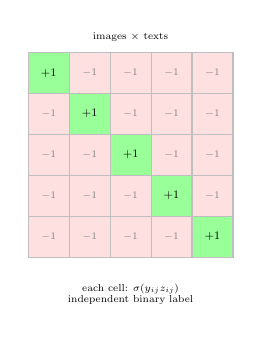
\begin{tikzpicture}[scale=0.52, every node/.style={scale=0.52}]
          \def\m{5}
          \foreach \i in {1,...,\m} {
            \foreach \j in {1,...,\m} {
              \pgfmathtruncatemacro{\d}{\i==\j ? 1 : 0}
              \ifnum\d=1
                \fill[green!40] ({(\j-1)}, {(\m-\i)}) rectangle ++(1,1);
                \node[font=\footnotesize] at ({\j-0.5},{\m-\i+0.5}) {$+1$};
              \else
                \fill[red!12] ({(\j-1)}, {(\m-\i)}) rectangle ++(1,1);
                \node[font=\scriptsize, gray] at ({\j-0.5},{\m-\i+0.5}) {$-1$};
              \fi
              \draw[gray!50] ({(\j-1)}, {(\m-\i)}) rectangle ++(1,1);
            }
          }
          \node[font=\scriptsize, anchor=south] at (\m/2, \m+0.15) {images $\times$ texts};
          \node[font=\scriptsize, align=center] at (\m/2,-0.9)
            {each cell: $\sigma(y_{ij}z_{ij})$ \\ independent binary label};
        \end{tikzpicture}
      \end{center}
    \end{column}
  \end{columns}

  \vspace{0.3em}
  \textbf{Consequences}: no cross-device all-gather (only block-wise dot products, easy to \emph{chunk} for memory); the objective is \emph{decoupled from batch size}, so it stays stable even at small batches. Catch: huge class imbalance ($N$ positives vs.\ $N^2{-}N$ negatives) needs a learnable bias (next slide).
\end{frame}

% -----------------------------------------------------------------------
\begin{frame}{SigLIP: The Sigmoid Loss}

  \begin{columns}
    \begin{column}{0.50\textwidth}
      For each pair $(i,j)$ in a batch of $N$ pairs, the logit and label are
      \[ z_{ij} = \tau\,\mathbf{I}_i\cdot\mathbf{T}_j + b, \qquad
         y_{ij} = \begin{cases} +1 & i=j \\ -1 & i\neq j \end{cases} \]
      \[ \mathcal{L}_{\text{SigLIP}} = -\frac{1}{N}\sum_{i=1}^{N}\sum_{j=1}^{N}
         \log \sigma\!\big(y_{ij}\,z_{ij}\big) \]

      \begin{itemize}
        \item $\tau=e^{t}$ and $b$ are \emph{single global} scalars; init $\tau{=}10$, $b{=}{-}10$
        \item The $\pm1$ label multiplies the \emph{whole} logit, so the one shared $b$ shifts positives and negatives in \emph{opposite} directions: a learned threshold encoding the prior ``most pairs are negative''
        \item At init $b{=}{-}10$ makes $\sigma\!\approx\!0$ everywhere, matching that prior, so the many negatives cause no huge initial gradient
        \item \textbf{No reweighting}: all $N^2$ terms count equally (sum $/N$); the bias, not a class weight, offsets the imbalance
      \end{itemize}
    \end{column}
    \begin{column}{0.48\textwidth}
      \begin{center}
        \begin{tikzpicture}[scale=0.85]
          \clip (-3.4,-0.6) rectangle (3.6,3.5);
          % axes
          \draw[-Stealth] (-3.2,0) -- (3.4,0) node[right, font=\scriptsize] {$z_{ij}$};
          \draw[-Stealth] (0,-0.3) -- (0,3.4) node[above, font=\scriptsize] {$-\log\sigma(y z)$};
          % positive pair: y=+1 -> loss = ln(1+e^{-z}); wants z large
          \draw[very thick, green!55!black, domain=-3:3, samples=80, smooth]
            plot (\x, {0.62*ln(1+exp(-2*\x))});
          % negative pair: y=-1 -> loss = ln(1+e^{z}); wants z small
          \draw[very thick, red!65, domain=-3:3, samples=80, smooth]
            plot (\x, {0.62*ln(1+exp(2*\x))});
          \node[green!45!black, font=\scriptsize, anchor=east] at (-0.3,2.9) {positive ($y{=}{+}1$)};
          \node[red!70!black, font=\scriptsize, anchor=west] at (0.3,2.9) {negative ($y{=}{-}1$)};
          \node[green!45!black, font=\tiny, anchor=west] at (1.4,0.55) {push $z\uparrow$};
          \node[red!70!black, font=\tiny, anchor=east] at (-1.4,0.55) {push $z\downarrow$};
        \end{tikzpicture}
      \end{center}
      {\scriptsize Per-pair logistic loss: matches are pushed to high $z$, mismatches to low $z$. The shared bias $b$ shifts both curves horizontally (a learned decision threshold), starting them where almost everything is classified negative.}
    \end{column}
  \end{columns}
\end{frame}

% -----------------------------------------------------------------------
\begin{frame}{SigLIP: Architecture and Training}

  \begin{columns}
    \begin{column}{0.55\textwidth}
      \textbf{ViT-So400m/14}: a \emph{shape-optimized} ViT from \cite{dehghani2023shape}.
      Instead of uniformly scaling depth/width, a compute-optimal search over depth, width, and MLP dimension finds a better shape for a given parameter budget.

      \vspace{0.3em}
      \begin{center}
      \scriptsize
      \begin{tabular}{l c c c c c}
        \toprule
        \textbf{Model} & \textbf{Depth} & \textbf{Width} & \textbf{Heads} & \textbf{MLP} & \textbf{Params} \\
        \midrule
        ViT-B/16  & 12 & 768  & 12 & 3072 & 86M  \\
        ViT-L/16  & 24 & 1024 & 16 & 4096 & 307M \\
        \textbf{So400m/14} & \textbf{27} & \textbf{1152} & \textbf{16} & \textbf{4304} & \textbf{428M} \\
        ViT-H/14  & 32 & 1280 & 16 & 5120 & 632M \\
        \bottomrule
      \end{tabular}
      \end{center}
      \vspace{0.1em}

      Note: MLP dim $= 3.74 \times$ width (not the standard $4\times$). The search finds a non-standard shape: more depth and width than ViT-L but a narrower MLP ratio, achieving better performance than ViT-H at fewer parameters.

      \vspace{0.2em}
      \textbf{Text encoder}: same shape as the image encoder (depth 27, width 1152). Fully symmetric two-tower design.
    \end{column}
    \begin{column}{0.43\textwidth}
      \textbf{Training}:
      \begin{itemize}
        \item \textbf{Dataset}: WebLI (Google's web-scraped image-text dataset), $\sim$10B pairs
        \item \textbf{Batch sizes}: from 1K to 1M; sweet spot at $N = 32{,}768$
        \item Resolution: $224 \times 224$, optionally fine-tuned at $384 \times 384$
        \item Shared embedding space dim: 1152 (= hidden width, no extra projection)
      \end{itemize}
    \end{column}
  \end{columns}
\end{frame}

% -----------------------------------------------------------------------
\begin{frame}{SigLIP: Results}

  \textbf{Zero-shot ImageNet top-1 accuracy}:
  \vspace{0.2em}

  \begin{columns}
    \begin{column}{0.48\textwidth}
      \begin{center}
      \scriptsize
      \begin{tabular}{l c c}
        \toprule
        \textbf{Model} & \textbf{Params} & \textbf{IN top-1} \\
        \midrule
        ResNet-50 (supervised) & 25M & 76.1\% \\
        CLIP ViT-L/14@336 & 428M & 76.2\% \\
        \midrule
        SigLIP B/16@256 & 86M & 76.7\% \\
        SigLIP L/16@256 & 307M & 80.5\% \\
        SigLIP L/16@384 & 307M & 82.1\% \\
        SigLIP So400m/14@224 & 428M & 82.2\% \\
        SigLIP So400m/14@384 & 428M & \textbf{83.2\%} \\
        \bottomrule
      \end{tabular}
      \end{center}
      {\scriptsize Publicly released checkpoints (trained far longer than the paper's batch-size ablations); numbers as tabulated in \cite{tschannen2025siglip2}.}
    \end{column}
    \begin{column}{0.48\textwidth}
      \begin{itemize}
        \item SigLIP B/16 already matches CLIP ViT-L/14 and supervised ResNet-50
        \item Shape-optimized So400m/14 pushes to \textbf{83.2\%} zero-shot
        \item Higher resolution at fine-tuning consistently helps (+1--2\%)
      \end{itemize}

      \vspace{0.3em}
      \begin{block}{From the paper itself}
        \footnotesize
        The original paper's headline is \emph{efficiency}: from-scratch SigLIP B/16 reaches \textbf{73.4\%} (batch 32K, 5 days on 32 TPUv4); SigLiT (locked image tower) hits \textbf{84.5\%} in 2 days on 4 chips.
      \end{block}
    \end{column}
  \end{columns}
\end{frame}

% -----------------------------------------------------------------------
\begin{frame}{SigLIP: Effect of Batch Size (Sigmoid vs.\ Softmax)}

  \vspace{0.2em}
  \begin{columns}
    \begin{column}{0.52\textwidth}
      \begin{center}
        \begin{tikzpicture}[scale=0.95]
          % axes
          \draw[-Stealth] (-0.3,0) -- (6.0,0);
          \draw[-Stealth] (0,-0.2) -- (0,3.5);
          \node[font=\scriptsize, rotate=90, anchor=south] at (-0.55,1.7) {ImageNet 0-shot};
          \node[font=\scriptsize, anchor=north] at (3.0,-0.55) {batch size (log scale)};
          % x ticks
          \foreach \x/\lab in {0/4K,1/8K,2/16K,3/32K,4/98K,5/307K} {
            \draw[gray!50] (\x,0) -- (\x,-0.08);
            \node[font=\tiny, anchor=north] at (\x,-0.1) {\lab};
          }
          % sweet-spot marker
          \draw[gray!55, dashed] (3,0) -- (3,3.2);
          \node[font=\tiny, text=gray!50!black, anchor=south] at (3,3.2) {sweet spot};
          % sigmoid curve (green)
          \draw[very thick, green!55!black, smooth] plot coordinates
            {(0,1.45) (1,2.05) (2,2.55) (3,2.9) (4,2.78) (5,2.3)};
          % softmax curve (red)
          \draw[very thick, red!65, smooth] plot coordinates
            {(0,0.72) (1,1.45) (2,2.12) (3,2.58) (4,2.72) (5,2.12)};
          % legend
          \draw[very thick, green!55!black] (3.6,1.15) -- (4.0,1.15);
          \node[font=\tiny, anchor=west] at (4.05,1.15) {sigmoid (SigLIP)};
          \draw[very thick, red!65] (3.6,0.75) -- (4.0,0.75);
          \node[font=\tiny, anchor=west] at (4.05,0.75) {softmax (CLIP)};
        \end{tikzpicture}
      \end{center}
      {\scriptsize Schematic redrawn from Fig.~2 (SigLIP, 9B examples); axes are qualitative.}
    \end{column}
    \begin{column}{0.46\textwidth}
      \begin{itemize}
        \item For batch $<16$K, sigmoid beats softmax by a \textbf{large margin}
        \item The gap closes as batch grows: \textbf{SigLIP peaks at 32K}; softmax needs 98K for its optimum and still does not surpass sigmoid
        \item Pushing further (307K, up to \textbf{1M} for SigLiT) \emph{hurts} both $\Rightarrow$ 32K is a practical sweet spot
        \item Same saturation for multilingual mSigLIP (Table~2: $\approx$73.2\% across 32K--128K)
        \item No all-gather / global denominator $\Rightarrow$ memory-efficient ``chunked'' loss enables batches up to 1M on few chips
      \end{itemize}
    \end{column}
  \end{columns}
\end{frame}

% =======================================================================
\subsection{PaliGemma}

% -----------------------------------------------------------------------
\begin{frame}{PaliGemma: A Versatile Vision-Language Model}

  \cite{beyer2024paligemma}: Combine a strong vision encoder (SigLIP) with a strong LLM (Gemma) via a \textbf{simple linear projection}.

  \vspace{0.2em}
  \begin{center}
    \begin{tikzpicture}[
      scale=0.82, every node/.style={scale=0.82},
      comp/.style={draw, rounded corners, minimum height=0.55cm, align=center, font=\small},
      arr/.style={-Stealth, thick},
      tok/.style={minimum width=0.44cm, minimum height=0.44cm, draw=gray!60,
                  inner sep=0pt, font=\tiny, line width=0.3pt},
    ]
      % ============================================================
      %  TOKEN SEQUENCE (middle row) — laid out first to set positions
      % ============================================================
      \def\toksep{0.48}
      \def\toksy{0}

      % Image tokens: indices 0..4, dots, 6  (7 slots)
      \foreach \i in {0,...,4} {
        \node[tok, fill=orange!25] at ({-4.2 + \i*\toksep}, \toksy) {};
      }
      \node[font=\tiny] at ({-4.2 + 5*\toksep}, \toksy) {$\cdots$};
      \node[tok, fill=orange!25] at ({-4.2 + 6*\toksep}, \toksy) {};

      % Text tokens: indices 7..10  (4 slots)
      \foreach \i in {7,...,10} {
        \node[tok, fill=cyan!25] at ({-4.2 + \i*\toksep}, \toksy) {};
      }

      % Output tokens: indices 11..14  (4 slots)
      \foreach \i in {11,...,14} {
        \node[tok, fill=green!25] at ({-4.2 + \i*\toksep}, \toksy) {};
      }

      % Output text labels inside the output tokens
      \node[font=\tiny, green!30!black, baseline, inner sep=0pt, anchor=base] at ({-4.2 + 11*\toksep}, {\toksy - 0.06}) {A\strut};
      \node[font=\tiny, green!30!black, baseline, inner sep=0pt, anchor=base] at ({-4.2 + 12*\toksep}, {\toksy - 0.06}) {dog\strut};
      \node[font=\tiny, green!30!black, baseline, inner sep=0pt, anchor=base] at ({-4.2 + 13*\toksep}, {\toksy - 0.06}) {on\strut};
      \node[font=\tiny, green!30!black, baseline, inner sep=0pt, anchor=base] at ({-4.2 + 14*\toksep}, {\toksy - 0.06}) {the\strut};
      \node[font=\small, green!50!black] at ({-4.2 + 15*\toksep}, \toksy) {$\cdots$};

      % Braces above token sequence (labeling each group)
      \draw[decorate, decoration={brace, amplitude=3pt}, thick, orange!70!black]
        ({-4.2 - \toksep/2 + 0.02}, {\toksy + 0.32}) -- ({-4.2 + 6*\toksep + \toksep/2 - 0.02}, {\toksy + 0.32})
        node[midway, above=4pt, font=\tiny, text=orange!70!black] {256 image tokens};

      \draw[decorate, decoration={brace, amplitude=3pt}, thick, blue!70!black]
        ({-4.2 + 7*\toksep - \toksep/2 + 0.02}, {\toksy + 0.32}) -- ({-4.2 + 10*\toksep + \toksep/2 - 0.02}, {\toksy + 0.32})
        node[midway, above=4pt, font=\tiny, text=blue!70!black] {prefix text};

      \draw[decorate, decoration={brace, amplitude=3pt}, thick, green!50!black]
        ({-4.2 + 11*\toksep - \toksep/2 + 0.02}, {\toksy + 0.32}) -- ({-4.2 + 14*\toksep + \toksep/2 - 0.02}, {\toksy + 0.32})
        node[midway, above=4pt, font=\tiny, text=green!50!black] {generated output};

      % ============================================================
      %  Derived x-centres for alignment
      % ============================================================
      \pgfmathsetmacro{\imgcx}{-4.2 + 3*\toksep}      % centre of image tokens
      \pgfmathsetmacro{\txtcx}{-4.2 + 8.5*\toksep}     % centre of text tokens
      \pgfmathsetmacro{\outcx}{-4.2 + 12.5*\toksep}    % centre of output tokens

      % ============================================================
      %  IMAGE BRANCH — on top, centred above image tokens
      %  Layout (top to bottom): image → SigLIP → Linear Proj → tokens
      % ============================================================
      \def\imgsize{1.4}
      \pgfmathsetmacro{\imgL}{\imgcx - \imgsize/2}
      \pgfmathsetmacro{\imgR}{\imgcx + \imgsize/2}
      % Position image at top
      \pgfmathsetmacro{\imgT}{5.0}
      \pgfmathsetmacro{\imgB}{\imgT - \imgsize}

      % Tikz "photo" with patch grid
      \begin{scope}
        \clip (\imgL, \imgB) rectangle (\imgR, \imgT);
        \fill[blue!25] (\imgL, \imgB) rectangle (\imgR, \imgT);
        \fill[green!35!brown!30] (\imgL, \imgB) rectangle (\imgR, {\imgB + 0.45});
        \fill[yellow!70!orange] ({\imgcx + 0.4}, {\imgT - 0.28}) circle (0.18);
        \fill[brown!60] ({\imgcx - 0.28}, {\imgB + 0.28}) rectangle ({\imgcx - 0.20}, {\imgB + 0.7});
        \fill[green!50!black] ({\imgcx - 0.24}, {\imgB + 0.68}) circle (0.2);
        \fill[brown!50] ({\imgcx + 0.20}, {\imgB + 0.28}) ellipse (0.18 and 0.11);
        \fill[brown!50] ({\imgcx + 0.36}, {\imgB + 0.36}) circle (0.08);
      \end{scope}
      \pgfmathsetmacro{\ps}{\imgsize / 4}
      \foreach \r in {0,...,3} {
        \foreach \c in {0,...,3} {
          \draw[white, line width=0.5pt, opacity=0.8]
            ({\imgL + \c*\ps}, {\imgB + \r*\ps}) rectangle ++({\ps}, {\ps});
        }
      }
      \draw[thick] (\imgL, \imgB) rectangle (\imgR, \imgT);
      \node[font=\tiny, text=gray, anchor=east] at ({\imgL - 0.1}, {\imgB + \imgsize/2}) {$16{\times}16$ patches};

      % SigLIP box — below image
      \node[comp, fill=orange!20, minimum width=1.8cm] (vit) at (\imgcx, {\imgB - 0.85}) {SigLIP ViT {\tiny (400M)}};
      \draw[arr] (\imgcx, \imgB) -- (vit);

      % Linear Proj — below SigLIP
      \node[comp, fill=green!15, minimum width=1.8cm] (proj) at (\imgcx, {\imgB - 1.95}) {Linear Proj.};
      \draw[arr] (vit) -- (proj);

      % Arrow from Linear Proj down to image tokens
      \draw[arr, orange!70!black] (proj) -- (\imgcx, {\toksy + 0.85});

      % ============================================================
      %  TEXT BRANCH — on top, centred above prefix text tokens
      % ============================================================
      \node[font=\scriptsize] (txtlabel) at (\txtcx, \imgT) {\textit{``Describe this image.''}};
      \node[comp, fill=cyan!10, minimum width=1.8cm] (tokenizer) at (\txtcx, {\imgT - 0.8}) {Tokenizer};
      \draw[arr] (txtlabel) -- (tokenizer);

      % Arrow from Tokenizer down to text tokens
      \draw[arr, blue!70!black] (tokenizer) -- (\txtcx, {\toksy + 0.85});

      % ============================================================
      %  GEMMA — wide block BELOW the token sequence
      % ============================================================
      \pgfmathsetmacro{\gemmaL}{-4.2 - \toksep/2 - 0.05}
      \pgfmathsetmacro{\gemmaR}{-4.2 + 14*\toksep + \toksep/2 + 0.05}
      \pgfmathsetmacro{\gemmaT}{\toksy - 0.85}
      \pgfmathsetmacro{\gemmaB}{\toksy - 1.55}

      \fill[cyan!12, rounded corners=4pt] (\gemmaL, \gemmaB) rectangle (\gemmaR, \gemmaT);
      \draw[thick, rounded corners=4pt] (\gemmaL, \gemmaB) rectangle (\gemmaR, \gemmaT);
      \node[font=\small] at ({(\gemmaL+\gemmaR)/2}, {(\gemmaB+\gemmaT)/2}) {\textbf{Gemma 2B} {\tiny (decoder-only)}};

      % Arrows: all input tokens feed down into Gemma
      \foreach \i in {0,...,4} {
        \draw[-Stealth, thin, orange!50!black, opacity=0.5]
          ({-4.2 + \i*\toksep}, {\toksy - 0.22}) -- ({-4.2 + \i*\toksep}, \gemmaT);
      }
      \draw[-Stealth, thin, orange!50!black, opacity=0.5]
        ({-4.2 + 6*\toksep}, {\toksy - 0.22}) -- ({-4.2 + 6*\toksep}, \gemmaT);
      \foreach \i in {7,...,10} {
        \draw[-Stealth, thin, blue!50!black, opacity=0.5]
          ({-4.2 + \i*\toksep}, {\toksy - 0.22}) -- ({-4.2 + \i*\toksep}, \gemmaT);
      }

      % Autoregressive: up arrow (Gemma -> token) slightly left, down arrow (token -> Gemma) slightly right
      \foreach \i in {11,...,14} {
        \draw[-Stealth, thick, green!50!black]
          ({-4.2 + \i*\toksep - 0.06}, \gemmaT) -- ({-4.2 + \i*\toksep - 0.06}, {\toksy - 0.22});
        \draw[-Stealth, thick, green!50!black]
          ({-4.2 + \i*\toksep + 0.06}, {\toksy - 0.22}) -- ({-4.2 + \i*\toksep + 0.06}, \gemmaT);
      }
      \node[font=\tiny, text=green!40!black, anchor=west] at ({-4.2 + 14*\toksep + \toksep/2 + 0.05}, {(\toksy - 0.22 + \gemmaT)/2}) {autoregressive};

      % ============================================================
      %  Bracket: input to Gemma (prefix)
      % ============================================================
      \draw[decorate, decoration={brace, amplitude=4pt, mirror}, thick, gray]
        ({-4.2 - \toksep/2 + 0.02}, {\toksy - 0.22 - 0.08}) -- ({-4.2 + 10*\toksep + \toksep/2 - 0.02}, {\toksy - 0.22 - 0.08})
        node[midway, below=5pt, font=\tiny, text=gray] {prefix};

    \end{tikzpicture}
  \end{center}

  \vspace{0.1em}
  \begin{itemize}
    \item \textbf{Total}: $\sim$3B parameters (400M vision + 2B language + linear projection)
    \item \textbf{Key design choice}: A simple linear connector suffices when both components are individually strong
  \end{itemize}
\end{frame}

% -----------------------------------------------------------------------
\begin{frame}{PaliGemma: Three-Stage Training}

  \begin{center}
    \begin{tikzpicture}[
      scale=0.85, every node/.style={scale=0.85},
      stage/.style={draw, rounded corners, thick, minimum width=3.0cm, minimum height=1.2cm, align=center, font=\small},
      arr/.style={-Stealth, very thick, gray},
    ]
      % Stage 1
      \node[stage, fill=orange!12] (s1) at (-4.0, 0) {\textbf{Stage 1}\\Unimodal\\Pretraining};
      % Stage 2
      \node[stage, fill=blue!12] (s2) at (0.0, 0) {\textbf{Stage 2}\\Multimodal\\Pretraining};
      % Stage 3
      \node[stage, fill=green!12] (s3) at (4.0, 0) {\textbf{Stage 3}\\Task-Specific\\Fine-Tuning};

      \draw[arr] (s1) -- (s2);
      \draw[arr] (s2) -- (s3);
    \end{tikzpicture}
  \end{center}

  \vspace{0.3em}
  \begin{description}[style=nextline]
    \item[Stage 1: Unimodal pretraining]
      SigLIP and Gemma are pretrained \emph{separately} on their respective data.
      \begin{itemize}
        \item SigLIP: contrastive (sigmoid) loss on image-text pairs
        \item Gemma: autoregressive next-token prediction on text
      \end{itemize}
    \item[Stage 2: Multimodal pretraining]
      Full model trained jointly on a large mixture of multimodal tasks (captioning, VQA, OCR, detection, \ldots).
      Vision encoder is \emph{unfrozen}.
      Resolution: $224 \times 224$ (256 image tokens).
      \begin{itemize}
        \item \textbf{Loss}: Purely autoregressive next-token prediction on \emph{suffix (output) tokens only}. No contrastive loss
        \item Image and prefix text tokens are excluded from the loss (prefix-LM masking)
        \item Gradients still flow into the vision encoder via backpropagation through the linear projection
      \end{itemize}
    \item[Stage 3: Task-specific fine-tuning]
      Fine-tune on individual downstream benchmarks. Same loss as Stage~2.
      \begin{itemize}
        \item Resolution can be increased: $448 \times 448$ ($\to$ 1024 tokens) or $896 \times 896$ ($\to$ 4096 tokens) for detail-oriented tasks (OCR, documents)
      \end{itemize}
  \end{description}
\end{frame}

% -----------------------------------------------------------------------
\begin{frame}{PaliGemma: Prefix-LM Attention Mask}

  \begin{columns}
    \begin{column}{0.55\textwidth}
      \begin{center}
        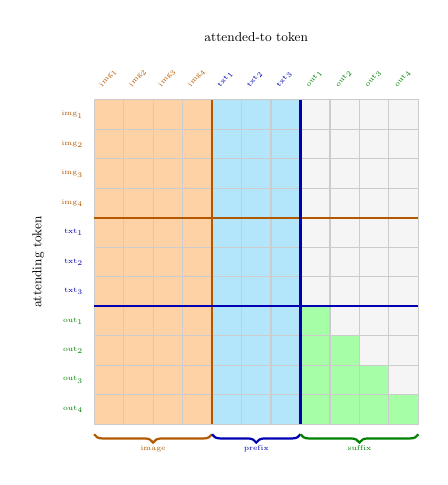
\begin{tikzpicture}[scale=0.52, every node/.style={scale=0.52}]
          % Dimensions: 4 image + 3 prefix + 4 suffix = 11
          \def\nimgtok{4}
          \def\npreftok{3}
          \def\nsuftok{4}
          \pgfmathtruncatemacro{\ntot}{\nimgtok+\npreftok+\nsuftok}
          \def\s{0.72}

          % Fill cells
          \foreach \row in {1,...,\ntot} {
            \foreach \col in {1,...,\ntot} {
              % Prefix region: rows 1..(nimgtok+npreftok), cols 1..(nimgtok+npreftok)
              \pgfmathtruncatemacro{\inprefix}{(\row<=\nimgtok+\npreftok) && (\col<=\nimgtok+\npreftok) ? 1 : 0}
              % Suffix causal: rows > (nimgtok+npreftok), col <= row
              \pgfmathtruncatemacro{\insuffcausal}{(\row>\nimgtok+\npreftok) && (\col<=\row) ? 1 : 0}
              % Suffix attending to prefix: rows > (nimgtok+npreftok), cols <= (nimgtok+npreftok)
              % Already covered by insuffcausal since col<=row and row>prefix end implies col<=row covers prefix cols too
              \pgfmathtruncatemacro{\attend}{\inprefix || \insuffcausal ? 1 : 0}
              \ifnum\attend=1
                % Color by region
                \pgfmathtruncatemacro{\isimg}{\col<=\nimgtok ? 1 : 0}
                \pgfmathtruncatemacro{\ispref}{(\col>\nimgtok) && (\col<=\nimgtok+\npreftok) ? 1 : 0}
                \pgfmathtruncatemacro{\issuf}{\col>\nimgtok+\npreftok ? 1 : 0}
                \ifnum\isimg=1
                  \fill[orange!35] ({(\col-1)*\s}, {(\ntot-\row)*\s}) rectangle ++(\s, \s);
                \fi
                \ifnum\ispref=1
                  \fill[cyan!30] ({(\col-1)*\s}, {(\ntot-\row)*\s}) rectangle ++(\s, \s);
                \fi
                \ifnum\issuf=1
                  \fill[green!35] ({(\col-1)*\s}, {(\ntot-\row)*\s}) rectangle ++(\s, \s);
                \fi
              \else
                \fill[gray!8] ({(\col-1)*\s}, {(\ntot-\row)*\s}) rectangle ++(\s, \s);
              \fi
              \draw[gray!40, thin] ({(\col-1)*\s}, {(\ntot-\row)*\s}) rectangle ++(\s, \s);
            }
          }

          % Row labels (left) — what token is attending
          \foreach \i in {1,...,\nimgtok} {
            \node[font=\tiny, anchor=east, text=orange!70!black] at (-0.15, {(\ntot-\i+0.5)*\s}) {img$_{\i}$};
          }
          \pgfmathtruncatemacro{\prefstart}{\nimgtok+1}
          \pgfmathtruncatemacro{\prefend}{\nimgtok+\npreftok}
          \foreach \i [evaluate=\i as \j using int(\i-\nimgtok)] in {\prefstart,...,\prefend} {
            \node[font=\tiny, anchor=east, text=blue!70!black] at (-0.15, {(\ntot-\i+0.5)*\s}) {txt$_{\j}$};
          }
          \pgfmathtruncatemacro{\sufstart}{\nimgtok+\npreftok+1}
          \foreach \i [evaluate=\i as \j using int(\i-\nimgtok-\npreftok)] in {\sufstart,...,\ntot} {
            \node[font=\tiny, anchor=east, text=green!50!black] at (-0.15, {(\ntot-\i+0.5)*\s}) {out$_{\j}$};
          }

          % Column labels (top) — what token is attended to
          \foreach \i in {1,...,\nimgtok} {
            \node[font=\tiny, rotate=50, anchor=south west, text=orange!70!black] at ({(\i-0.5)*\s-0.1}, {\ntot*\s+0.1}) {img$_{\i}$};
          }
          \foreach \i [evaluate=\i as \j using int(\i-\nimgtok)] in {\prefstart,...,\prefend} {
            \node[font=\tiny, rotate=50, anchor=south west, text=blue!70!black] at ({(\i-0.5)*\s-0.1}, {\ntot*\s+0.1}) {txt$_{\j}$};
          }
          \foreach \i [evaluate=\i as \j using int(\i-\nimgtok-\npreftok)] in {\sufstart,...,\ntot} {
            \node[font=\tiny, rotate=50, anchor=south west, text=green!50!black] at ({(\i-0.5)*\s-0.1}, {\ntot*\s+0.1}) {out$_{\j}$};
          }

          % Region separators
          \draw[thick, orange!70!black] (0, {(\ntot-\nimgtok)*\s}) -- ({\ntot*\s}, {(\ntot-\nimgtok)*\s});
          \draw[thick, orange!70!black] ({\nimgtok*\s}, 0) -- ({\nimgtok*\s}, {\ntot*\s});
          \draw[thick, blue!70!black] (0, {(\ntot-\nimgtok-\npreftok)*\s}) -- ({\ntot*\s}, {(\ntot-\nimgtok-\npreftok)*\s});
          \draw[thick, blue!70!black] ({(\nimgtok+\npreftok)*\s}, 0) -- ({(\nimgtok+\npreftok)*\s}, {\ntot*\s});

          % Axis labels
          \node[font=\small, rotate=90, anchor=south] at (-1.1, {\ntot*\s/2}) {attending token};
          \node[font=\small, anchor=south] at ({\ntot*\s/2}, {\ntot*\s+1.3}) {attended-to token};

          % Braces at top for regions
          \draw[decorate, decoration={brace, amplitude=3pt, mirror}, thick, orange!70!black]
            (0, -0.25) -- ({\nimgtok*\s}, -0.25) node[midway, below=4pt, font=\tiny] {image};
          \draw[decorate, decoration={brace, amplitude=3pt, mirror}, thick, blue!70!black]
            ({\nimgtok*\s}, -0.25) -- ({(\nimgtok+\npreftok)*\s}, -0.25) node[midway, below=4pt, font=\tiny] {prefix};
          \draw[decorate, decoration={brace, amplitude=3pt, mirror}, thick, green!50!black]
            ({(\nimgtok+\npreftok)*\s}, -0.25) -- ({\ntot*\s}, -0.25) node[midway, below=4pt, font=\tiny] {suffix};
        \end{tikzpicture}
      \end{center}
    \end{column}
    \begin{column}{0.43\textwidth}
      \textbf{Prefix-LM masking}:
      \begin{itemize}
        \item \textcolor{orange!70!black}{\textbf{Image}} + \textcolor{blue!70!black}{\textbf{prefix text}} tokens: \textbf{bidirectional} attention (full block)
        \item \textcolor{green!50!black}{\textbf{Suffix (output)}} tokens: \textbf{causal} attention (lower triangle)
        \item Suffix tokens attend to all prefix tokens + causally to previous suffix tokens
      \end{itemize}

      \vspace{0.3em}
      \textbf{Loss masking}:
      \begin{itemize}
        \item Loss computed \emph{only} on \textcolor{green!50!black}{\textbf{suffix}} tokens
        \item Image and prefix tokens are excluded
        \item Gradients still flow into the vision encoder via backpropagation
      \end{itemize}

      \vspace{0.3em}
      {\small Colored cells = attention allowed.\\
      Gray cells = masked (no attention).}
    \end{column}
  \end{columns}
\end{frame}

% -----------------------------------------------------------------------
\begin{frame}{PaliGemma: Tasks and Capabilities}

  PaliGemma handles diverse vision-language tasks through \textbf{text prompts}:

  \vspace{0.3em}
  \begin{center}
  \small
  \begin{tabular}{l l l}
    \toprule
    \textbf{Task} & \textbf{Prompt} & \textbf{Output} \\
    \midrule
    Captioning & \texttt{caption en} & ``A dog running on the beach'' \\
    VQA & \texttt{What color is the car?} & ``red'' \\
    Object detection & \texttt{detect dog} & \texttt{<loc0123><loc0456>...~dog} \\
    OCR & \texttt{ocr} & Extracted text from image \\
    \bottomrule
  \end{tabular}
  \end{center}

  \vspace{0.5em}
  \begin{columns}
    \begin{column}{0.48\textwidth}
      \textbf{Object detection via text}:
      \begin{itemize}
        \item Bounding boxes encoded as special \texttt{<loc>} tokens
        \item Normalized coordinates in $[0, 1023]$
        \item No task-specific detection head needed
      \end{itemize}
    \end{column}
    \begin{column}{0.48\textwidth}
      \textbf{Why this works}:
      \begin{itemize}
        \item All tasks unified as text generation
        \item No task-specific architectures
        \item Same model, different prompts
        \item Higher resolution for detail-oriented tasks (OCR, documents)
      \end{itemize}
    \end{column}
  \end{columns}
\end{frame}

% -----------------------------------------------------------------------
\begin{frame}{PaliGemma: Benchmark Results}

  PaliGemma (3B) vs.\ larger VLMs after task-specific fine-tuning. Bold = best in column.

  \vspace{0.3em}
  \begin{center}
  \resizebox{\textwidth}{!}{%
  \begin{tabular}{l c c | c c c c c c c}
    \toprule
    \textbf{Model} & \textbf{Size} & \textbf{Res.} & \textbf{VQAv2} & \textbf{TextVQA} & \textbf{DocVQA} & \textbf{ChartQA} & \textbf{AI2D} & \textbf{SciQA} & \textbf{GQA} \\
    \midrule
    LLaVA-1.5     & 7B  & 336  & 78.5  & 58.2  & --    & --    & --    & 66.8  & 62.0 \\
    LLaVA-1.5     & 13B & 336  & 80.0  & 61.3  & --    & --    & --    & 71.6  & 63.3 \\
    Qwen-VL-Chat  & 10B & 448  & 78.2  & 61.5  & 65.1  & 65.7  & 62.3  & 68.2  & 57.5 \\
    \midrule
    PaliGemma     & 3B  & 224  & 83.2  & 55.5  & 43.7  & 57.1  & 72.1  & 95.4  & 65.6 \\
    PaliGemma     & 3B  & 448  & \textbf{85.6}  & 73.2  & 78.0  & 71.4  & \textbf{73.3}  & \textbf{95.9}  & \textbf{67.0} \\
    PaliGemma     & 3B  & 896  & --    & \textbf{76.5}  & \textbf{84.8}  & --    & --    & --    & -- \\
    \bottomrule
  \end{tabular}
  }
  \end{center}

  \vspace{0.2em}
  {\scriptsize SciQA = ScienceQA (image subset). All PaliGemma numbers from \cite{beyer2024paligemma}.}

  \vspace{0.3em}
  \begin{itemize}
    \item 3B model outperforms LLaVA-1.5-13B on most benchmarks
    \item \textbf{Resolution is critical}: DocVQA jumps from 43.7 (224px) to 84.8 (896px)
  \end{itemize}
\end{frame}

% -----------------------------------------------------------------------
\begin{frame}{PaliGemma: OCR, Captioning \& Localization}

  \vspace{-0.3em}
  \textbf{OCR \& text-heavy benchmarks}:
  \vspace{0.2em}

  \begin{center}
  \small
  \begin{tabular}{l c | c c c c}
    \toprule
    \textbf{Model} & \textbf{Res.} & \textbf{OCR-VQA} & \textbf{ST-VQA} & \textbf{InfoVQA} & \textbf{TallyQA\textsuperscript{s/c}} \\
    \midrule
    PaliGemma-3B     & 224  & 73.2  & 63.3  & 28.5   & 81.7\,/\,69.6 \\
    PaliGemma-3B     & 448  & 75.6  & 81.8  & 40.5   & 84.9\,/\,72.3 \\
    PaliGemma-3B     & 896  & \textbf{75.9}  & \textbf{84.4}  & \textbf{47.8}   & -- \\
    \bottomrule
  \end{tabular}
  \end{center}

  \vspace{0.3em}
  \textbf{Captioning \& referring expression segmentation}:
  \vspace{0.2em}

  \begin{center}
  \small
  \begin{tabular}{l c | c c | c c c}
    \toprule
    \textbf{Model} & \textbf{Res.} & \textbf{COCO\textsuperscript{CIDEr}} & \textbf{TextCaps\textsuperscript{CIDEr}} & \textbf{RefCOCO} & \textbf{RefCOCO+} & \textbf{RefCOCOg} \\
    \midrule
    PaliGemma-3B & 224 & 141.9  & 127.5  & 73.4  & 68.3  & 67.7 \\
    PaliGemma-3B & 448 & \textbf{144.6}  & \textbf{153.9}  & 75.6  & 69.8  & 70.2 \\
    PaliGemma-3B & 896 & --     & --     & \textbf{76.9}  & \textbf{72.2}  & \textbf{72.2} \\
    \bottomrule
  \end{tabular}
  \end{center}

  \vspace{0.2em}
  {\scriptsize RefCOCO metrics: Mean IoU. TallyQA\textsuperscript{s/c} = simple/complex split.}

  \vspace{0.3em}
  \begin{block}{Design Lessons}
    \begin{enumerate}
      \item A \textbf{simple linear connector} suffices when both vision encoder and LLM are strong
      \item \textbf{Resolution matters}: cheap to increase at fine-tuning, large gains on detail-oriented tasks
      \item \textbf{Unified text generation} handles captioning, VQA, detection, OCR without architectural changes
    \end{enumerate}
  \end{block}
\end{frame}

% =======================================================================
\subsection{Summary}

% -----------------------------------------------------------------------
\begin{frame}{Multimodal Models: Summary}

  \textbf{Evolution of vision-language models}:

  \vspace{0.3em}
  \begin{center}
    \begin{tikzpicture}[
      scale=0.8, every node/.style={scale=0.8},
      model/.style={draw, rounded corners, thick, minimum width=2.8cm, minimum height=0.8cm, align=center, font=\small},
      arr/.style={-Stealth, very thick, gray!60},
    ]
      \node[model, fill=orange!15] (clip) at (-3.5, 0) {\textbf{CLIP} (2021)\\Contrastive alignment};
      \node[model, fill=violet!12] (siglip) at (0.5, 0) {\textbf{SigLIP} (2023)\\Sigmoid loss};
      \node[model, fill=green!15] (pali) at (4.5, 0) {\textbf{PaliGemma} (2024)\\Generative VLM};

      \draw[arr] (clip) -- (siglip) node[midway, above, font=\scriptsize] {better loss};
      \draw[arr] (siglip) -- (pali) node[midway, above, font=\scriptsize] {+ LLM};
    \end{tikzpicture}
  \end{center}

  \vspace{0.5em}
  \begin{columns}
    \begin{column}{0.48\textwidth}
      \textbf{CLIP}:
      \begin{itemize}
        \item Dual encoder, shared embedding space
        \item Softmax contrastive loss (InfoNCE)
        \item Zero-shot classification via text prompts
        \item Cannot generate text
      \end{itemize}
    \end{column}
    \begin{column}{0.48\textwidth}
      \textbf{PaliGemma}:
      \begin{itemize}
        \item SigLIP vision encoder + Gemma LLM
        \item Simple linear projection connector
        \item Generates text conditioned on images
        \item Unified interface for captioning, VQA, detection, OCR
      \end{itemize}
    \end{column}
  \end{columns}

  \vspace{0.3em}
  \textbf{Key insight}: Contrastive pretraining produces excellent visual features. Pairing them with a language model unlocks generative capabilities far beyond embedding comparison.
\end{frame}
